\chapter*{Organization Focus}
\label{chap:Organization_focus}
% Esempi
% bla \cite{some_label}
% Referenza Pagina \pageref{sec:origine}
% Referenza \ref{sec:origine}
The ``AllSpark Informatic Company''\footnote{Also defined during the document as ``Company''.} is a fancy medium organization in the Information Technology business that we have in mind in order to analyze the Information Systems around it. Its life in the market is strictly bound to the service through WEB, but it also provides Software programs reselling and associate consultant. The main scope of the present analysis is to formalize the company business in order to improve the efficiency, incresing the quality given to customers and growing the profit.


Due to the continue growing of Web applications and the increasingly predominance of the Internet itself, the Company has fully assured his future to the Network in any treated aspects. The service it offers are about the hosting, storing, security, software reselling and developing, consulting and involving certifications. By the physical view, this company is distribuited on the countries and can have several employees in all around the world comunicating through the same services develeped by the internal programmers.


The company is strongly oriented to research and developing optimal solutions in order to fit the high quality requests from customers. Moreover it is involved with Foundations to get Free Software and it joins the Free Software philosophy contributing in bug tracing, patching and development of software it works with.


To offer noticeable features and satisfy the customers there is a Section with particular interest in fulfilment standards, laws appliance and discovery new fashion trends.


A very important section is the ``Research and Development'' section which works around new technologies, fresh ideas and updating existing solutions in order to offer to customers support, updates and terrific new features.



\chapter{Organization modeling}
\label{chap:Organization_modeling}
In order to model the AllSpark to a complete organizational analysis is suggested to adopt the Zachman framework. The following analysis are going to focus the only first two rows of the forecast model to achieve the first representation of the ``case study'' business.

\section{Scope}
\label{sec:Scope}
The ``Scope'' row allows to describe the Context in which the enterprise works. In the AllSpark is going to be an analysis of the environment which characterizes the people working inside, the mission goals, the expected business functions, the informations exchanged whithin the company and finally a brief description of the operating method during the time.

\subsection{People (Who)}
\label{subsec:scope[People]}
In this column are represented the entity interested on the company's business activity. In the AllSpark perspective there are several stakeholders that are involved in the enterprise's functions:
\begin{itemize}
 \item {\bf Customers:} the Company's lymph, are enterprises or private consumer which are searching products that satifies their target;
 \item {\bf Banks:} financial organization which are directly involved in the Company's business;
 \item {\bf Foundations:} the AllSpark collaborates with the Free Software Foundation, Mozilla et.al. because it belives in the mutual growing of the software it is using;
 \item {\bf Universities:} are cultural institution which work on advanced education;
 \item {\bf Course participants:} are other companies' workers or private people that receive education about some topic which AllSpark is certificate to;
 \item {\bf Govern:} is the geographical Country the Company should respect laws;
 \item {\bf Consultants:} external professional skilled people contacted by AllSpark in order to get information which it does not hold;
 \item {\bf Supplier:} company that provide any kind of equipment to the Company;
 \item {\bf ISP:} (Internet Service Provide) company that allow the connection of the Company to the Internet;
\end{itemize}

The relations between the entities just listed are modeled through the i* diagrams reported in figure \ref{img:i_star}. The goals of the main actors of the previous cited model are shown in figure \ref{img:internal_goals}.



\begin{figure}
\centering
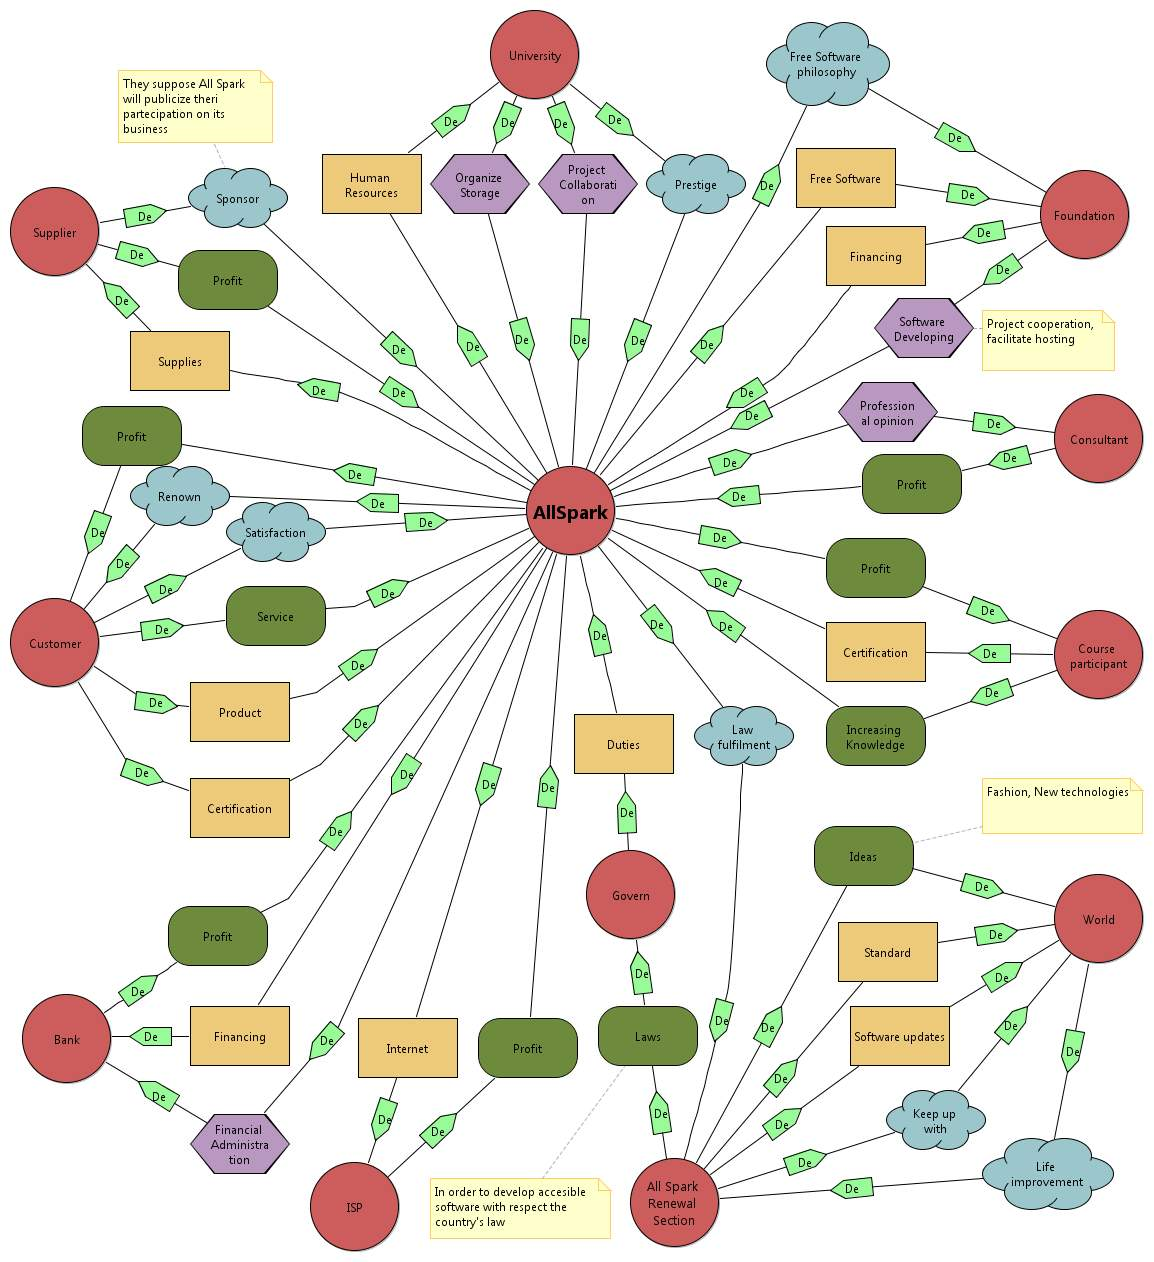
\includegraphics[scale=0.45]{Si_star/img/i_star_vertical}
\caption{Relationship between actors regarding AllSpark.}
\label{img:i_star}
\end{figure}


\begin{figure}
\centering
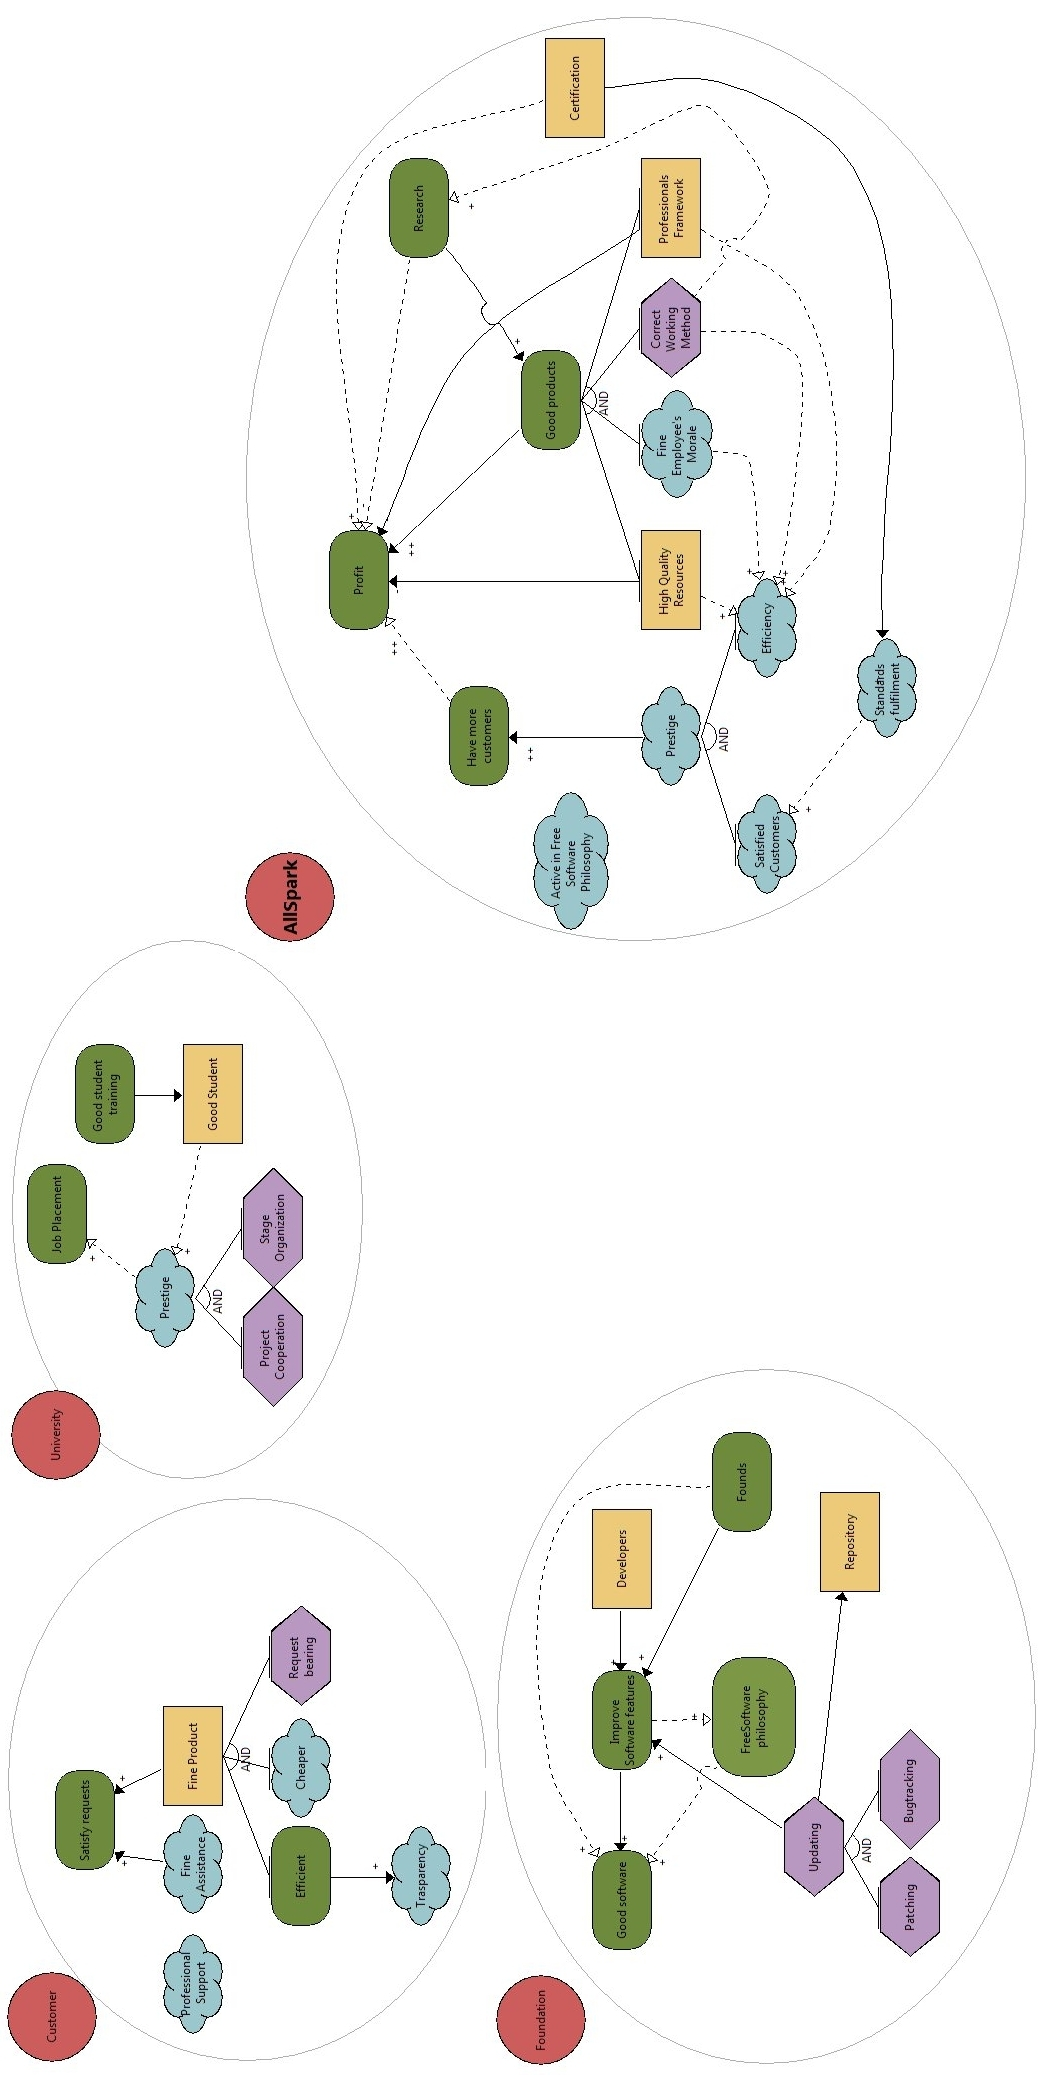
\includegraphics[scale=0.28]{Si_star/img/internal_goals}
\caption{Main actor goals.}
\label{img:internal_goals}
\end{figure}

\subsection{Motivation (Why)}
\label{subsec:scope[Motivation]}
Each entity in the Company aims to reach some objective in order to contribute at the global success. This section illustrate the AllSpark goals through the single internal actors' goals which concurrent on the global Company one. The follow list explain what are these objective in which entities are involved:
\begin{itemize}
 \item {\bf Organization itself (this):} first of all the AllSpark is interested on profit, image and growing sales. In order to do that the Company aim to satisfy others objective that are reliability, quality and efficiency. Moreover the Company is going to be involved on the Free Software perspective and it should want manage its resources in order to supply the philosophy;
 \item {\bf Customer:} he is looking for service hosting, network security, data storage, consultation in order to supply his business processes basing on supplied functions;
 \item {\bf Supplier:} he provides the hardware and the software the Company depends on. Additionally he supplies licences that permits the Company to manage;
 \item {\bf Bank:} as a credit institute, the bank is interested on give financial services, loan, sponsorship in exchange of a fee;
 \item {\bf Foundation:} the primary scope of Foundation is to find funds to destinate on the research and development software. It is also interested on spread the Free Software philosophy and search collaboration with companies in order to give software and have as return cooperation of bugtracking\footnote{When a bug is discovered it is sended to the Foundation in order to have knowledge.} and, eventually, patching\footnote{It's even possible that programmers provide some patches to send to the Foundation in order to contribute the Opensource Projects.}), support it\footnote{It may be possible hosting a mirror site or instantiate a collaborative work area};
 \item {\bf University:} organize stage, prestige, job placement;
 \item {\bf Course participant:} grow knowledge, get certification, improving skills;
 \item {\bf Consultant:} increse reputation(renown), profit;
\end{itemize}

\subsection{Functions (How)}
\label{subsec:scope[Functions]}
In the following section are showed the organization's processes that characterize the company profile across the real world. Each function has to be well defined in order to avoid overlaps and so defining a robust and efficient working structure that may support the business growth during the years.
\begin{itemize}
  \item {\bf Service hosting:} AllSpark offers resources and several technology service in order to satisfy the customers' requests of having a service on the Web. The scope of the function is to permit to organizations or private developers to appear on the Web as they wish. There are different kind of offers categorized by: bandwidth, space and elaboration usage, kind of services needed, kind of services developed, level of warranty, reliability and quality expected by client;
  \item {\bf Security system implementation:} a customer may require some particular security bounderies on his service or a newer one offered by AllSpark and so the scope of the function is to fit them at best. The Company plawns to manage the software and hardware resources trasparently to the range of customer's application even if the customer's system is hosted by it.
  \item {\bf Data storage:} the Company offers to customers to have some remote space useful for their business accessible through several standard protocols or some ones developed by the AllSpark itself in order to assure the service. The function forseen different kind of parallel services to fit the customer expectation in terms of quality, guarantee, efficiency, reliability and privacy;
  \item {\bf Consulting:} AllSpark is oriented in given consulting to organizations in order to support their business in the best way. This implies that the consulting may be also in the services that it is offering or some new features just introduced;
% 	\subitem \textit{hiring a consultant};
% 	\subitem \textit{support customer decision};
  \item {\bf Organize course:} given that the professional skilled figure inside the Company grow with interesting experience and apply standard which they are trained for, comes naturally that AllSpark wants to be enabled to release certifications covering the educational role;
%   \item {\bf Certification:};
% 	\subitem \textit{getting};
% 	\subitem \textit{giving};
  \item {\bf Payment:} of course each company needs to be payed for its work and this function includes both the receiving payment and the giving payment to external entity that occur in the AllSpark's business;
  \item {\bf Billing:} in order to fit the right corrispective of the tasks done it's necessary to calculate with particular attention to the concurrent companies and to maximize the profit calculate with high precision the effective work;
  \item {\bf Foundation support:} since the AllSpark is involved in the Free Software philosophy is right to participate in the software evolution it depends on. So it is important the method adopted by the employee in order to report the bug first and to starting a task force to develop a possibile patch if the analysis coming from the bug trace reveals a simple solution;
  \item {\bf External collaboration:} some customers may require a complex project that needs cooperation with others professionists. In particular the Company may require external analysts or give the partial developer of the project to a third company;
\end{itemize}

\paragraph{}
Figure \ref{img:secur} describes how a customer deals with
AlSpark in order to implement a security system in their 
enterprise.
The workflow is divided into three phases, the first regards
requirements analysis: here the customer can purchase some 
hardware devices which are needed in order to complete the
system.

Then, during the developing phase, AllSpark releases periodically
a beta version of the system, which will be tested with the customer's
support in order to fine-tune the requirements.

Finally when the system is completely operative, AllSpark install
the definitive version on the customer machines. 

\paragraph{}
In figure \ref{img:certs} is described the procedure followed for
taking part in formation courses in order to take certification of
quality as sysadmin or developer.

The AllSpark policy regarding the courses is that a customer has 
two possibility of taking the exam each time he subscribes to the
course. 

\begin{figure}
\centering
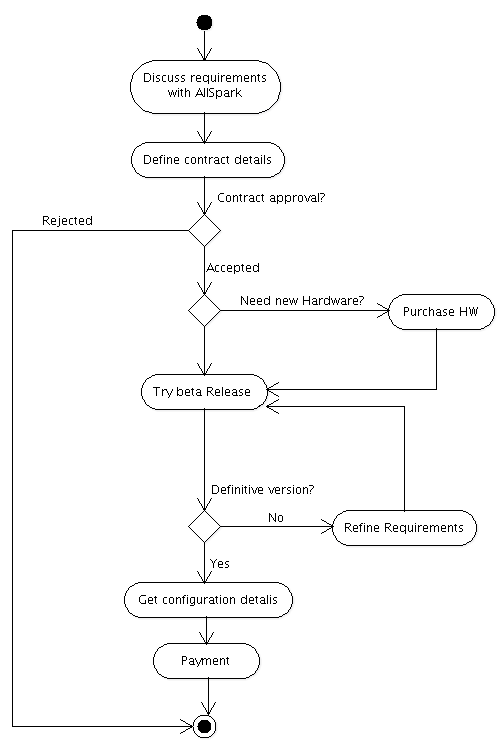
\includegraphics[scale=0.70]{argouml_diags/imgs/secur}
\caption{Workflow of project development}
\label{img:secur}
\end{figure}

\begin{figure}
\centering
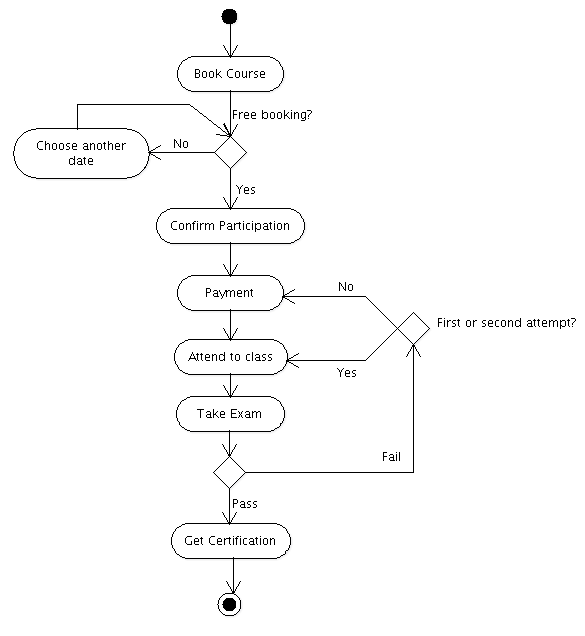
\includegraphics[scale=0.75]{argouml_diags/imgs/certs}
\caption{Procedure followed for getting certifications}
\label{img:certs}
\end{figure}



\subsection{Data (What)}
\label{subsec:scope[Data]}
The ``Data'' are the elements inside the company used in order to manage the internal resources, support project developing, making strategic decision, supporting advertising campaign and so on. Since the organization work in the I.T. sector, it tends to have digital-kind documents in order to improve the retriveral efficiency and decrease the management expenses. There are several kind of data which help to understand the function's scope and the enterprise's workflow.
\begin{itemize}
  \item {\bf Resource:} in this kind of document are explicited the basic information about the element whithin the Company such as servers, printers, terminals and so on;
% 	\subitem \textit{URI};
% 	\subitem \textit{Name};
% 	\subitem \textit{Description};
% 	\subitem \textit{Revision Changelog};
  \item {\bf Course:} reports the complete description about the course the company is involved in. In particular are signed the scheduling of the lectures, the location foreseen to run, the certificates for which it supply to and the lecturers charged to perform the lecture;
% 	\subitem \textit{Name};
% 	\subitem \textit{Schedule};
% 	\subitem \textit{Description};
% 	\subitem \textit{Localization};
% 	\subitem \textit{Certificate};
% 	\subitem \textit{Lecturer};
  \item {\bf Customer list:} it is simply a sequence of organization of private names that have a business contract with AllSpark;
  \item {\bf Supplier list:} all the supplier that have been contacted by the Company during the years are mantained in a single historical detailed list;
  \item {\bf Partners list:} are the companies which are interested on the good success of the AllSpark. In particular they may be cooperate company or simple the financial institution that give funds to projects developed by;
  \item {\bf Software:} in order to effcient manage the developed software it is important to know some fundamentals information like current selling version, the licence given, current selling price and the customers' advises inherent in it;
% 	\subitem \textit{Name};
% 	\subitem \textit{Description};
% 	\subitem \textit{Version};
% 	\subitem \textit{Licence};
% 	\subitem \textit{Price};
% 	\subitem \textit{Customer suggest};
  \item {\bf Hardware:} the document contains the fully technical specifications about every hardware component equipped on the company's system and relative notes about some potential issues in order to facilitate the emergency substitution of faults components;
% 	\subitem \textit{Internal ID};
% 	\subitem \textit{Model};
% 	\subitem \textit{Technical specifications};
% 	\subitem \textit{Issues};
  \item {\bf Connection:} since the Company works all the business through Internet several comunication lines are working at and a detailed list made up of the number of own lines, Internet Service Providers, technical specifications and fees permits to efficiently manage borderline cases;
% 	\subitem \textit{Internal ID};
% 	\subitem \textit{Internet Service Provider};
% 	\subitem \textit{Technical specifications};
% 	\subitem \textit{Fee};
  \item {\bf Supplier/Order:} is a list reporting the orders sent by Company to its supplier that contains a tracking number, the location of expected order, the foreseen arrival time and the object quantity;
% 	\subitem \textit{ID};
% 	\subitem \textit{Supplier};
% 	\subitem \textit{Location};
% 	\subitem \textit{Arrival time};
% 	\subitem \textit{Quantity};
  \item {\bf Contracts:} all the business agreement that AllSpark has taken with the customers. The document contain;
% 	\subitem \textit{Customer};
% 	\subitem \textit{Data};
% 	\subitem \textit{Details};
% 	\subitem \textit{Value};
  \item {\bf Financial data:} in order to make strategic decisions is essential to analyze real, updated and historical financial information about the expected Company's evolution. This kind of data are also similar to the Financial Management data that are deeply interested on the current financial status of the Company. Again similar are the profit data that incorporate the projection of the profit of the last semester and last year;
  \item {\bf Projects:} the core of the Company and of its future projection. This document is essential to the AllSpark's growth given that it contains fundamental informations about the involved people, the roles occupied by who, eventually associate partners and additional informations characteristics to the Project, that may be a research project or a commercial product project, about the Project Management;
% 	\subitem \textit{Type\footnote{R\&D or ``Product''}};
% 	\subitem \textit{Staff involved};
% 	\subitem \textit{Partners};
% 	\subitem \textit{Resources};
% 	\subitem \textit{Certification};
% 	\subitem \textit{Details\footnote{such documents related, starting time, milestones etc.}};
  \item {\bf Certifications:} list of all the certifications achieved by the organization and their historical information such as agreement date and expiring date and finally details that permit to contextualize the certificate's field of application;
% 	\subitem \textit{Name};
% 	\subitem \textit{Agreement Date};
% 	\subitem \textit{Expiring Date};
% 	\subitem \textit{Details};
  \item {\bf Workers:} list of the employees enrolled in the AllSpark with relative informations about salary, owned skills, efficiency and specialization concerning job. This is useful to have a efficient Project Management placing the right person in the right position with right team;
% 	\subitem \textit{Name};
% 	\subitem \textit{Salary};
% 	\subitem \textit{Skills};
% 	\subitem \textit{Efficiency};
% 	\subitem \textit{Specialization};
  \item {\bf Advice campign:} a significant informations about the advice campaigns are useful in order to improve future ones. The data collected in the document are inherent the media adopted, the involved temporal time, the supported costs, the expected objective to achieve and finally the end report about the campaign efficency and quality;
% 	\subitem \textit{ID};
% 	\subitem \textit{Data issued};
% 	\subitem \textit{Media};
% 	\subitem \textit{Starting date};
% 	\subitem \textit{Ending date};
% 	\subitem \textit{Costs};
% 	\subitem \textit{Objectives};
% 	\subitem \textit{Efficiency and quality};
  \item {\bf Statistical report:} contains informations about the market analysis, network management, hardware management and the AllSpark efficiency and performance status in order to make strategic decision about given facts;
% 	\subitem \textit{Efficiency and Performance};
% 	\subitem \textit{Market};
% 	\subitem \textit{Network management};
% 	\subitem \textit{Hardware management};
%   \item {\bf Profit:} the kind of information ;
% 	\subitem \textit{Semester};
% 	\subitem \textit{Value};
  \item {\bf Network monitoring:} this is a kind of report specialized on real time network monitoring in order to detect enventually abnormalities in the standard operating flow;
\end{itemize}

\begin{figure}
\centering
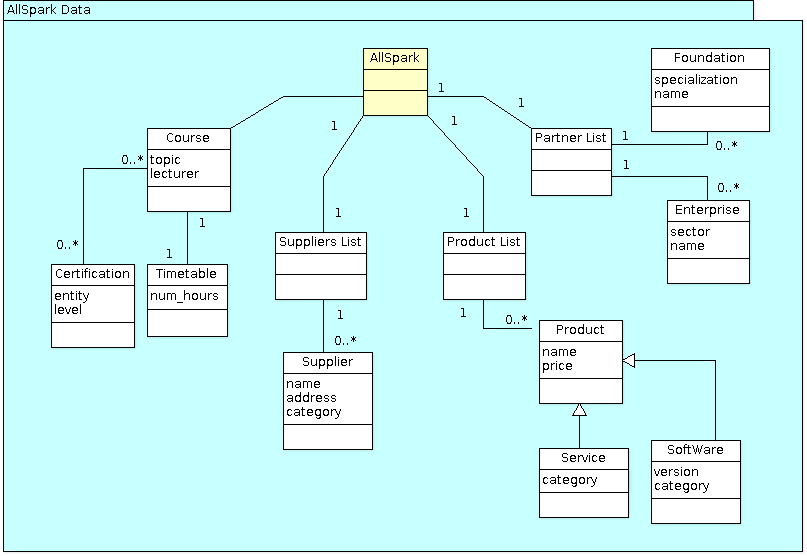
\includegraphics[scale=0.70]{argouml_diags/imgs/data}
\caption{Class diagram representing the relevant data}
\label{img:data1}
\end{figure}



\subsection{Time (When)}
\label{subsec:scope[Time]}
At this level Time is considered as description of the business cycle and the business events that trigger some actions. The ordinary company's lifecycle forecast eight hours per day working for a five days week. However the services the company is supplying are always active for twentyfour hour per day for three hundred and sixtyfive days per year, hence there is a fundamental distinction about what employees do and what the Company is effectively giving. Of course some faults may happen, but the Company is prepared to face thanks a meticulous plan developed in order to guarantee to customer the optimal service.


In order to provide an efficient service there are some particular case the AllSpark has to consider may happen, in particular the events that characterize some primary actions are:
\begin{itemize}
  \item {\bf Hardware fault:} it's well known that each physical component has a lifetime over which the broke's likelihood grow, but more trivial may be a simple imperfect component that brokes even though it's new. The whole system is studied to minimize the negative impact and default procedural assure, if the replacement components are on the AllSpark store, the suitable repair in few hours without affecting the global functionality.
% 	\subitem \textit{repair:} In the case of faulty is important to recognize quickly the harm and provide the right substitution procedure. Moreover is interesting adopt some security mechanism in order to avoid systems' downtime;
  \item {\bf Service down:} for several reasons a service may go down, in particular after an update, a hardware or security fault, a ISP cutting down line and an another service configuration. If the ill service does not come from an external entity, bearing in mind the efficiency, the functionality is restored having a short technical analysis to isolate the problem followed by the appropriate resolving procedure;
% 	\subitem \textit{repair};
  \item {\bf Security fault:} all the services offered are avaiable through the Internet and even though the continue improvements and researches done by the employees to mantain the system secure and usable it may happen that someone can force the defenses. Hence it's important recognize the issue and perform a security analysis in order to raise the defence if the existing defensive shield is bypassed.
% 	\subitem \textit{security analysis};
  \item {\bf Project late:} due requirement changing or developing issues a project should acquire delay. When it exceeds the prefixed boundary, if the responsible can realize the issue, is necessary to study the causes and eventually reengineer the project to restore the efficiency;
% 	\subitem \textit{project analysis};
  \item {\bf ISP down:} a dangerous issue that compromise the work and for which the Company cannot resolve is the Internet cut line. If AllSpark owns a backup line with a different provider, the best tradeoff is the load balancing through the several Internet connection of different ISP;
% 	\subitem \textit{load balancing};
\end{itemize}

\subsection{Network (Where)}
\label{subsec:scope[Network]}
The contextual's Network cell define information about the locations where the enterprise operates. The nature of the business that AllSpark is performing leads to the opportunity of centralize the entire Organizational phisical structure in a single building. This improve the inter-comunication about the different section of the Company and facilitate the cooperation project. The Company owns an entire building which hosts both the employees and the systems and the comunications with the third party take place usually by Internet or telephone. In order to better manage the customers' relation the representative has the objective to personally see the the applicant and friendly discuss about his requirements and the company's proposal.


All the other relations depend on the third party's context and are not well defined a priori.


A very noticeable note is about the ``where'' the work is done by the AllSpark; the most of the work is performed on the systems inside the building that are projected to the World through the Internet, so it is particular important the connectivity which permits to be ``everywhere'' at the same time. In order to be specific clear the Organization claims some rights about itself names, hosted names and Internet adresses to figure unique in the World, hence a lot of URI collected by the company in several years have to be constantly renewed and updated.


% =================
% Enterprise model, 2^ Row Zachman framework
% =================

\section{Enterprise Model}
\label{sec:Enterprise}
The ``Enterprise Model'' row permits to define the nature of the business. In particular in this layer is interesting to see in more detail the internal structure of the ``case study'' organization used to modelling the business model adopted by the AllSpark in order to make an abstract representation of its internal processes.

\subsection{People (Who)}
\label{subsec:enterprise[People]}
In this second level of ``People'' are analyzed the internal actors of the Company.
\begin{itemize}
 \item {\bf Programmers:} are software developers skilled on programming, personalizing software configurations and services, bugfixes, patching, updating and so on;
 \item {\bf Sysadmins:} they work directly on the hardware systems, operative systems and connectivity;
 \item {\bf Administrative staff:} work in the company's lifecycle to make strategic decisions. In this staff there are: CEO, secretaries, business consultants, area managers;
 \item {\bf Representatives:} people that are charged to mantain the network contacts and are the public face of the Company;
 \item {\bf Analysts:} internal professional skilled people that have experience on projects and very good knowledge about software, project management;
\end{itemize}

The figure \ref{img:hierarchy} represent the complete AllSpark's hierarchy in order of understanding the internal relations among the personnel.

\begin{figure}
\centering
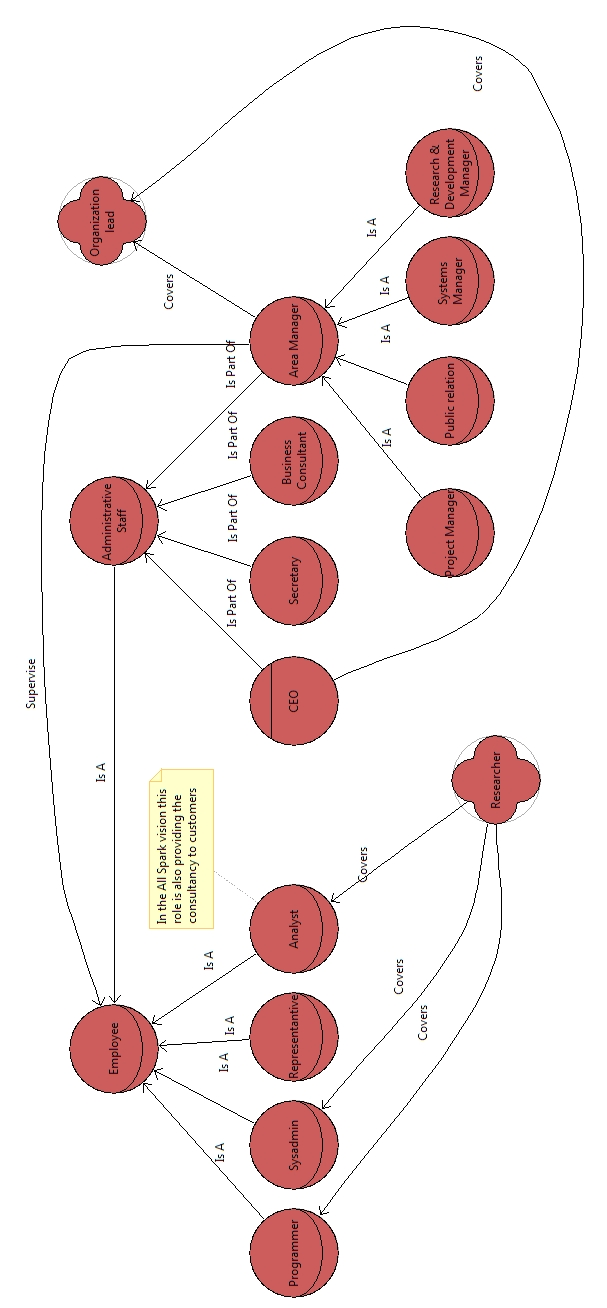
\includegraphics[scale=0.42]{Si_star/img/hierarchy}
\caption{AllSpark internal hierarchy.}
\label{img:hierarchy}
\end{figure}

\subsection{Motivation (Why)}
\label{subsec:enterprise[Motivation]}
The innerside of the AllSpark permit to analyze the single components as separated working entities.


Since the different facets of the business, it turns naturally that the internal entities lead to different perspective goals in particular each one has its own:
\begin{itemize}
 \item {\bf Programmer:} he focalize his job in implementing required solutions using his experience and working skills. Other important goals are doing research if he is enrolled in the research team and system maintenance whenever he looks to manage the running products;
 \item {\bf Sysadmin:} the primary target of this guy is to maintain the systems in order to take it reliable. Moreover is an essential figure to support the programmers preparing and for that is necessary the collaboration with them and so forth is important the quality assurance, a task always evolving due the updates;
 \item {\bf Administrative staff:} all the member in the staff are oriented to improve AllSpark's renown and performing strategic decision. Even more are involved in the human resource management to regulate and survey the personnel status and in the support to marketing analysis and operational;
 \item {\bf Representative:} is the public face of the Company to customers and first of all they aim to be good-looking. They always search for new  contracts, promoting products and services and finally their role is to manage contacts network accordingly with the Administrative staff;
 \item {\bf Analyst:} the primary goal he aims is manage the project. It's a really important goal since it includes all the project phases starting from the analysis. He's responsible about the project lifecycle\footnote{He supervise all the phases: requirement analysis, feasibility analysis, scheduling, milestones, testing and so on.} and its deployment;
\end{itemize}

\begin{figure}[!ht]
\centering
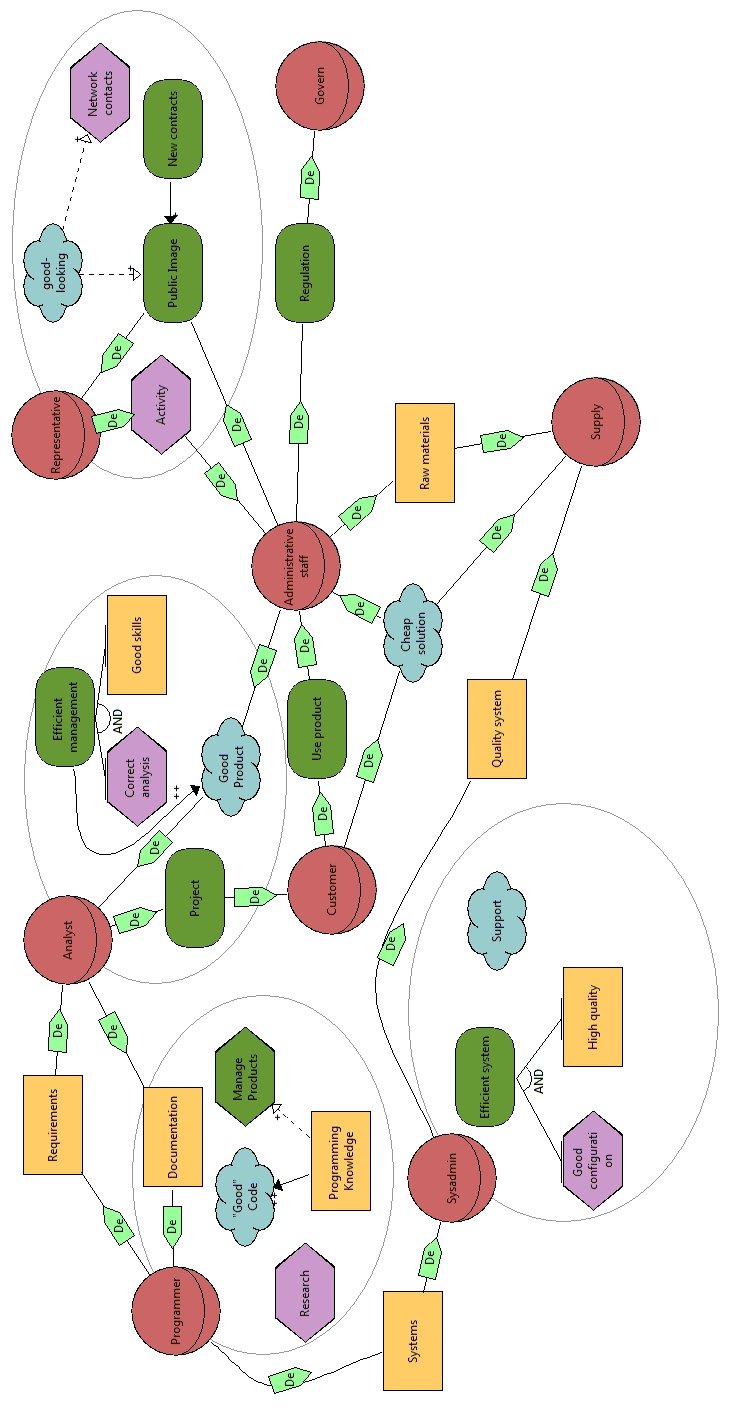
\includegraphics[scale=0.40]{Si_star/img/internal_goals_dependencies}
\caption{Diagram representing the internal dependencies}
\label{img:motiv2}
\end{figure}


\subsection{Functions (How)}
\label{subsec:enterprise[Functions]}
In this kind of level are presented the internal functions of Company's interest and that are involved in the business process. These functions are realized trasparently to external entities but they bring direct support to the effective functions seen in section \ref{subsec:scope[Functions]}.
\begin{itemize}
  \item {\bf Project management:} set of tasks grouped to administrate resources, timing, milestones, starting and closing procedure related to the Project's life;
  \item {\bf Human Resource Management:} is a core function interested on hiring, discharging, promoting, supporting, licensing, training and checking the AllSpark personnel;
  \item {\bf Supply management:} group of tasks which focus attention on the equipment: from the daily usage one to the complex system appliance;
  \item {\bf Finance management:} a good finance management assure the Company's growth and improving, so a good job of billing, investiments, promoting and budgets contributes in the global success;
  \item {\bf Licence management:} to continue operate in the usual way, or adopting new resources, is necessary pay attention on the licenses and their expiration date to avoid delays, damages or additional costs;
  \item {\bf Law appliance:} the scope is to fit the Country's requirements and to fit the implicit customer requirement, a noticeable attention should be taken over the law regulating the life inside the political boundaries. Even the virtual judgment on the Web should be followed in order to guarantee the client a reliable service;
  \item {\bf Burocracy aspect:} a very important task that permit the Company's regular activity in the Country environment. This task also include the contracts with customers, the cooperation agreements and so on;
  \item {\bf Updating software\&hardware:} in order to offer better services the AllSpark has to costantly check of software updates and the status of owned hardware. Its growth depends from the efficiency of resources adopted;
  \item {\bf Testing:} is the task that achieves to check the new developed product or an existential product that may be overhauled;
  \item {\bf Quality check:} during the project developing, a series of check guarantee the Company that the work flows in the right direction fulfils the contract with the customer;
  \item {\bf Service personalization:} given a third party, or a own developed, program is necessary to tune the features accordingly with the customers' need;
  \item {\bf Market analysis:} this function assure the company to be competitive with the other sector's companies, analyzing the costs, technology fashions and the product offered;
  \item {\bf Research:} is a complex task which enroll a lot of employees in order to develop new innovative product, find bugs, work on a patch, update developed softwares, improve security systems, perform software optimization, adopting standard specifications;
  \item {\bf Public relationship:} for the Company is useful have some experts who mantain friendly relations with customers and provide in searching for the new ones;
  \item {\bf Tuition fee payment:} as every other company, AllSpark has to pay other companies from which obtain services and in particular the Country is seen as a company;
\end{itemize}

In figure \ref{img:analysis} is described the first phase of a project,
regarding requirements analysis, as seen form AllSpark inside perspective.
Figures \ref{img:allocate} and \ref{img:gathering} explain in details the 
subprocesses called from the main process.
These, respectively, describe the procedure followed for allocate
a project and the relation between AllSpark and the consumer while collecting 
the requirements for the project.
\paragraph{}
Figure \ref{img:deploy} illustrates the business process which covers the last
phase of a project development: the effective deployment of the product.


\begin{figure}
\centering
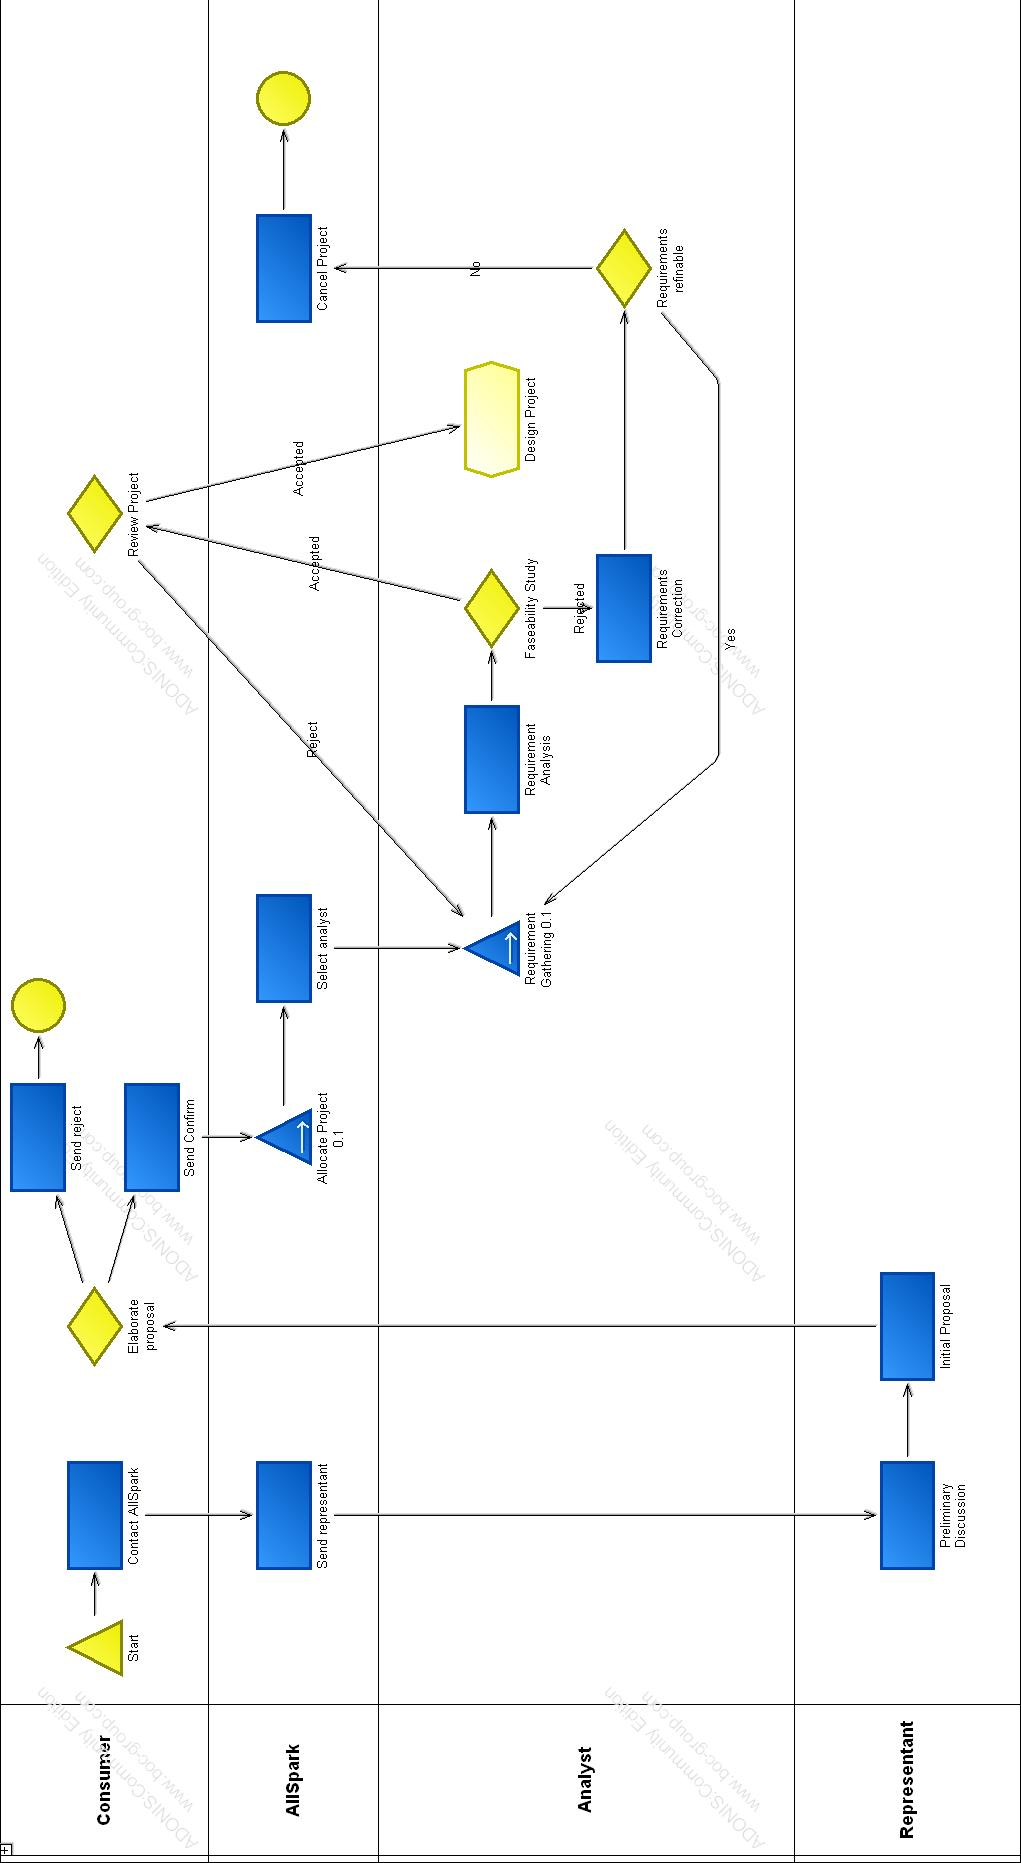
\includegraphics[scale=0.30]{adonis_diagrams/analysis}
\caption{Business process describing the first phase of a project development}
\label{img:analysis}
\end{figure}

\begin{figure}
\centering
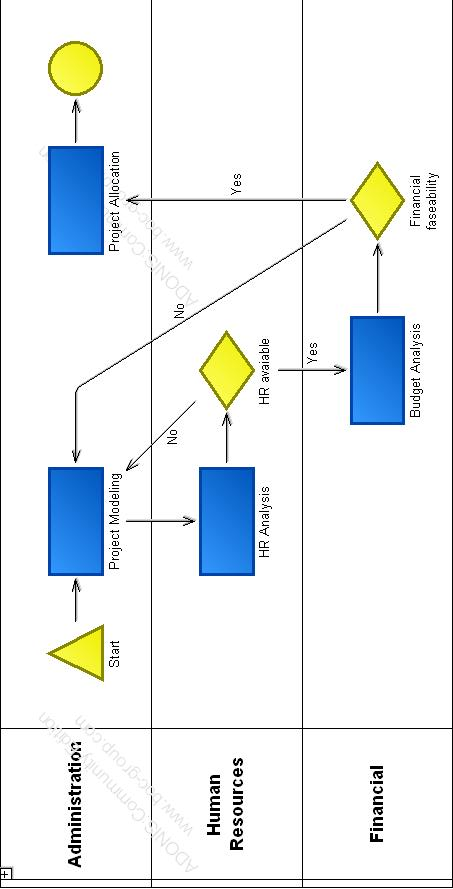
\includegraphics[scale=0.50]{adonis_diagrams/allocate}
\caption{AllSpark procedure for project allocation}
\label{img:allocate}
\end{figure}

\begin{figure}
\centering
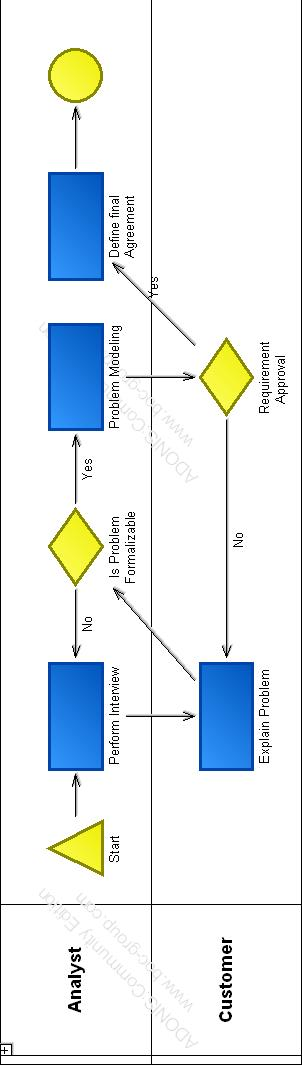
\includegraphics[scale=0.50]{adonis_diagrams/gather}
\caption{AllSpark procedure for requirements gathering}
\label{img:gathering}
\end{figure}

\begin{figure}
\centering
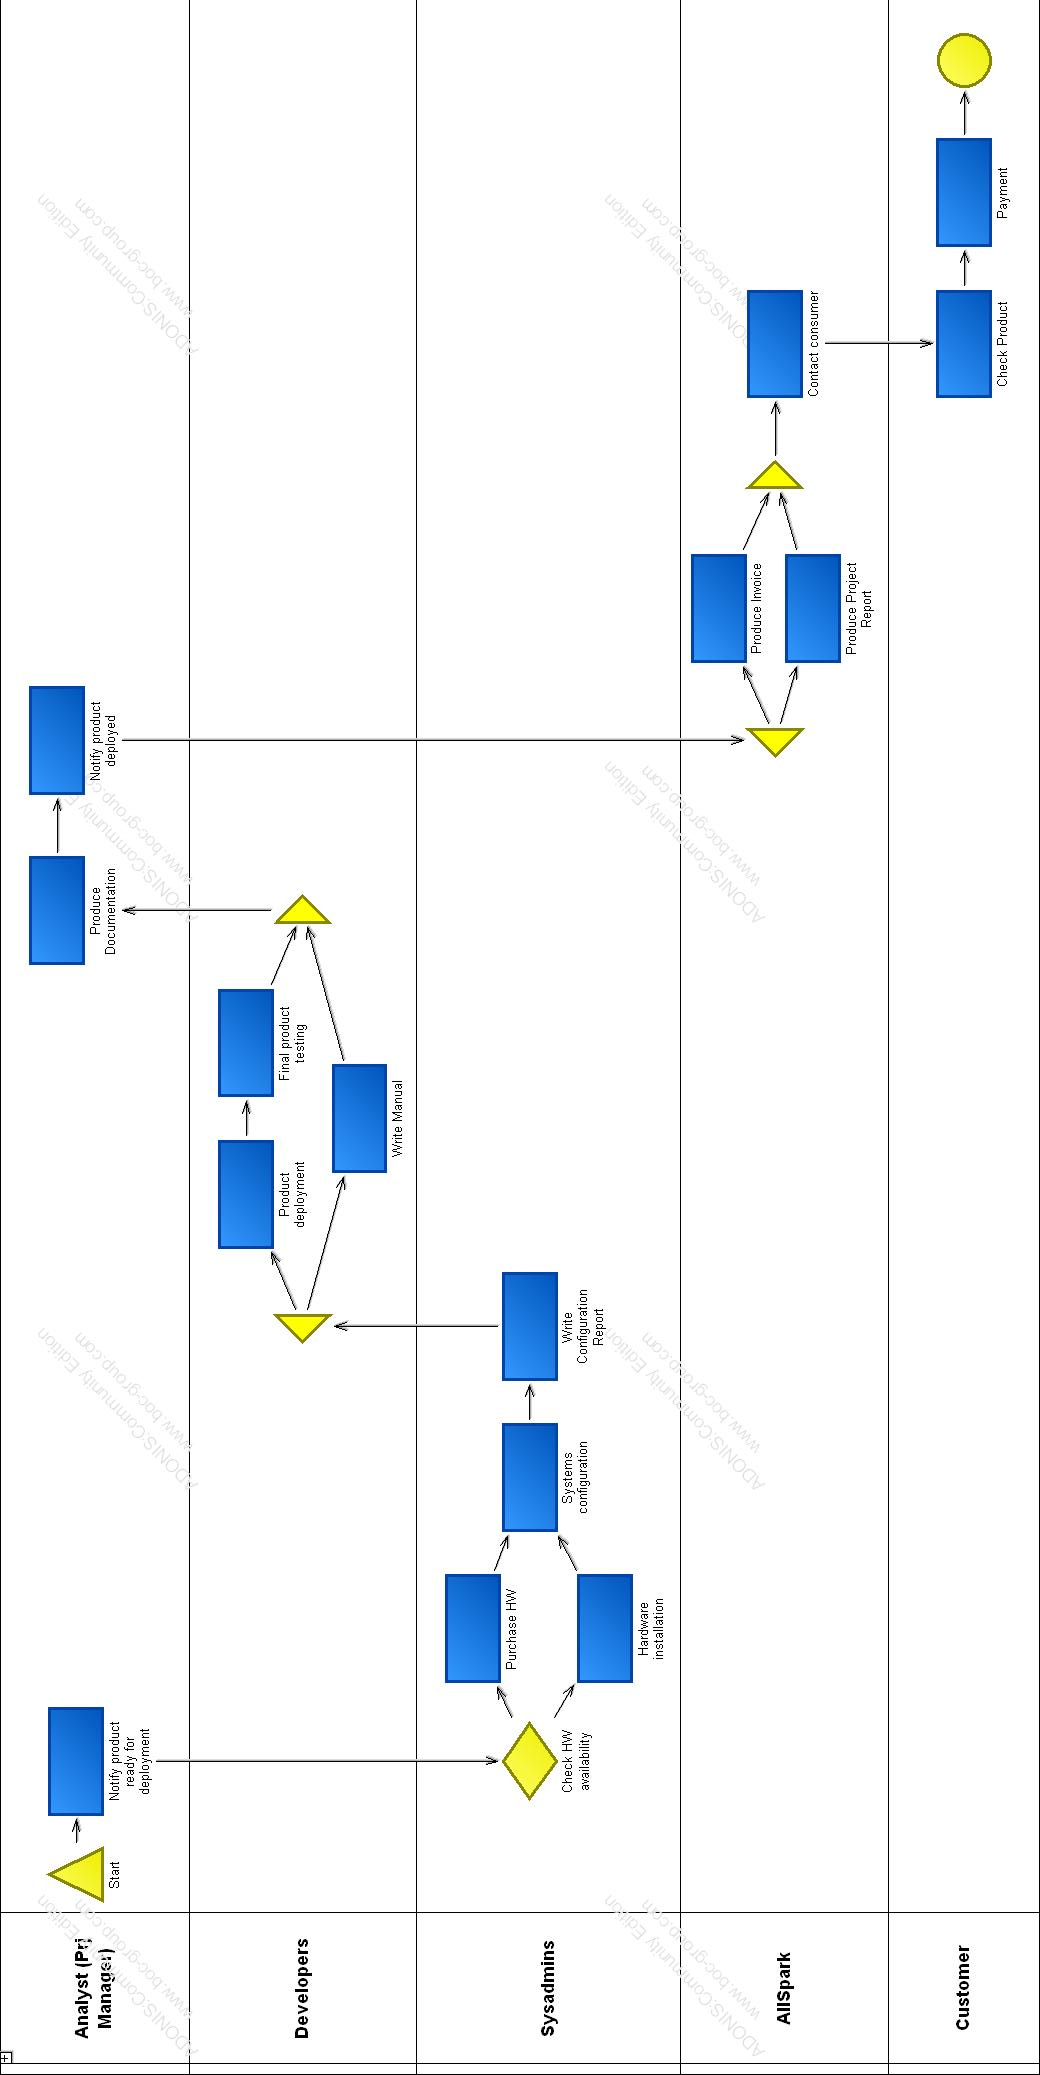
\includegraphics[scale=0.27]{adonis_diagrams/deploy}
\caption{Deploying of a project}
\label{img:deploy}
\end{figure}


\subsection{Data (What)}
\label{subsec:enterprise[Data]}



The internal structure, describing the relevant data need for AllSpark in
order to reach its goals, can be resumed in this list:
\begin{itemize}
\item {\bf Employee:} Allspark has some different kind of employees, 
they are divided mainly into Developers, Sysadmins, Analysts and Administration
staff.
\item {\bf Suppliers:} Our organization has to rely on different suppliers as
Hardware supplier, Software Supplier and Connectivity supplier.
\item {\bf Project:} The projects in which AllSpark is involved, are divided
in two categories, Security System or Service hosting.
\item {\bf Customer:} Another kind of useful data is the collection of our 
customer with relative contracts.
\item {\bf Partner:} AllSpark works in collaboration with organization of 
various kind, they can be Universities, Opensource Foundations and external 
consultants.
\end{itemize}

The class diagram in figure \ref{img:data2} can describe more efficiently  
the main data on which our organization works.

%\begin{figure}[!ht]
%\centering
%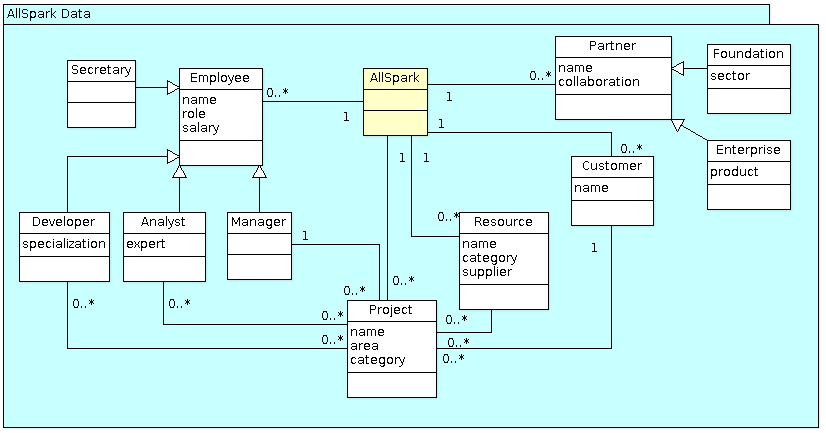
\includegraphics[scale=0.57]{argouml_diags/imgs/data2}
%\caption{Class diagram representing the relevant internal data}
%\label{img:data2}
%\end{figure}

%The internal structure, describing the relevant data need for AllSpark in
%order to reach its goals, can be resumed in this list:
%\begin{itemize}
%\item {\bf Employee:} Allspark has some different kind of employees, 
%they are divided mainly into Developers, Sysadmins, Analysts and Administration
%staff.
%\item {\bf Suppliers:} Our organization has to rely on different suppliers as
%Hardware supplier, Software Supplier and Connectivity supplier.
%\item {\bf Project:} The projects in which AllSpark is involved, are divided
%in two categories, Security System or Service hosting.
%\item {\bf Customer:} Another kind of useful data is the collection of our 
%customer with relative contracts.
%\item {\bf Partner:} AllSpark works in collaboration with organization of 
%various kind, they can be Universities, Opensource Foundations and external 
%consultants.
%\end{itemize}
%
%The class diagram in figure \ref{img:data2} can describe more efficently
%the main data on which aur organization works.
%
\begin{figure}[!ht]
\centering
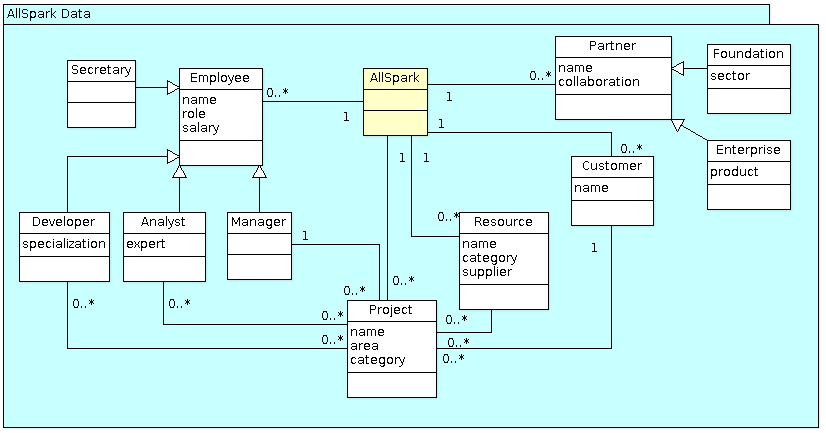
\includegraphics[scale=0.63,angle=90]{argouml_diags/imgs/data2}
\caption{Class diagram representing the relevant internal data}
\label{img:data2}
\end{figure}



\subsection{Time (When)}
\label{subsec:enterprise[Time]}
Since there are different areas that may cooperate, it is also necessary have weekly meeting with the relative area manager and the administrative staff. In particular there are some meeting needed to check the current state of the company business and they can be every month or semestral. Meetings are important in order to track the employees' jobs, to bear projects advancing, to analyze statistical reports, to shot the company status and finally to make strategic decisions.

Regarding the events coming from \ref{subsec:scope[Time]}, there is direct correspondence at this level that is build as they are since the elements affecting the internal personal are the same that affect the outside people and the actions involved are common to resolve the issues.


\begin{itemize}
  \item {\bf New Project started:} once the customer commit a work instance is necessary to evaluate the dimension of it through a complete deep analysis of the matter. If the Project receives the definitive approval by the CEO, a series of steps provide a complete allocating of resources starting from the human resources and ending with hardware and software ones needed.
% 	\subitem \textit{start};
  \item {\bf Salary\_day reached:} during the last month's week the the employees have right to receive the regular payment that should be calculated opportunely for each person based upon the enroll contract and the extra hours effectively worked if they have respected the contract;
% 	\subitem \textit{get\_salary};
  \item {\bf Project closed:} when a project reaches the endline, a couple of tasks have to be activated to conclude the activity. If the CEO accept the closure, then start unallocating the resources and the analysis of the project in order to improve the methods, the skills for the future ones and understanding the mistakes if the project is aborted or store the partial work done if it should be used in other projects;
% 	\subitem \textit{project analysis};
  \item {\bf Found a bug:} during the usual working process may happen some software error. Since the AllSpark is using a lot of free software and belives in its principles, after a brief analysis a warning report is sent to the software's developers. In the free software mind the code is easily distribuited and so a deep analysis may take place. If it reveals that the problem can be patched by an internal team, then a new internal project start in order to fix the problem. It's quite difficult manage the resource for a project of this kind and so an endterm is set to bound the costs;
% 	\subitem \textit{track bug};
% 	\subitem \textit{can be patched?};
% 		\subsubitem \textit{patch it};
  \item {\bf New Technology developed:} all around the world there are standardizing groups, Web developers and so on that publish new technology which influence the Web. If the Company's status is good, then AllSpark foreseen update meeting each six months in which the employees can fill the gap followed thanks external consultant who exposes the news.
\end{itemize}

\subsection{Network (Where)}
\label{subsec:enterprise[Network]}
The Network column indicates the locations where functions are expleted. In the ``case study'' the company has the lucky to be in a single big building where all the people work together in personal contact. Of course there are distinctions about different area into the building that permit efficient and ordered working flow based on the scope's area. In particular there are the following ones:
\begin{itemize}
  \item {\bf Administrative};
  \item {\bf Research};
  \item {\bf Development};
  \item {\bf Public relations};
  \item {\bf Systems};
\end{itemize}


Since all the comunication inside the building happens in the real world or through virtual systems the only specification to give are concerning the internal virtual method of comunication. The linking stuff is pretty technical, but generalizing is possible consider that each element is potentially connected to all the others.
% \begin{center}
%  \begin{tabular} {| c | p{20mm} | c | p{20mm} || p{40mm} |}
%   \hline
%   1st Column\footnote{footnote} & 2nd Column & 3rd Column \\
%   \hline
%   \end{tabular}
% \end{center}

% \begin{figure}[h]
%   \centering
%   \includegraphics[scale=0.85]{./immagini/image.pdf}
%   \caption{Description\label{fig:VoIP}}
% \end{figure}

% \begin{landscape}
% \begin{figure}[hbp]
%  \centering
%  \includegraphics[width=20cm,bb=0 0 1341 793]{img/people.png}
%  % people.png: 1788x1058 pixel, 96dpi, 47.30x27.99 cm, bb=0 0 1341 793
%  \caption{Relationships among external actors}
%  \label{fig:people_ext}
% \end{figure}
% \end{landscape}
